\documentclass[11pt]{article}

% \pagestyle{empty}                       %no page numbers
% \thispagestyle{empty}                   %removes first page number
\setlength{\parindent}{0in}               %no paragraph indents

\usepackage{fullpage}
\usepackage[tmargin = 0.5in, bmargin = 1in, hmargin = 1in]{geometry}     %1-inch margins
\geometry{letterpaper}                  
\usepackage{graphicx}
\usepackage{amssymb}

% Default packages
\usepackage{latexsym}
\usepackage{amsfonts}
\usepackage{amsmath}
\usepackage{amsthm}
\usepackage{hyperref}
\usepackage{fancyhdr}
\usepackage{enumitem}
\usepackage{pifont}

\newcommand{\cuthere}{%
\noindent
\raisebox{-2.8pt}[0pt][0.75\baselineskip]{\small\ding{34}}
\unskip{\tiny\dotfill}
}

\def\ra{\rightarrow}
\def\blank{\underline{\hspace{1in}}}

\def\pageturn{\vfill 
\begin{flushright}
	\begin{small}
		Continued $\ra$
	\end{small}
\end{flushright} \newpage}


\begin{document}
	
	\thispagestyle{empty}
	\renewcommand{\headrulewidth}{0.0pt}
	\thispagestyle{fancy}
	\lhead{Prof. Talbert}
	\chead{MTH 201: Calculus 1}
	\rhead{October 24/25, 2013}
	\lfoot{}
	\cfoot{}
	\rfoot{}	
	
	\vspace*{0in}

		\begin{center}
			\begin{large}
			\textbf{Class Activities: Using derivatives to describe families of functions} \\
			\end{large}
		\end{center}
	
Get into groups of 2--4 and work through all of the following activities. These are not to be turned in, and they will not be graded. Instead, record your group's work on your copy and keep it for notes. I will be coming to each group one by one as you work to observe what you're doing, answer questions, and catch any misconceptions that are happening. We will stop with about 10 minutes remaining to debrief the main ideas.

\section{Focus questions}

\begin{itemize}
	\item If $f'(a) > 0$, then $f$ is \blank at $x=a$. 
	\item If $f'(a) < 0$, then $f$ is \blank at $x=a$. 
	\item If $f''(a) > 0$, then $f$ is \blank at $x=a$.
	\item If $f''(a) <  0$, then $f$ is \blank at $x=a$.
\end{itemize}

\section{A one-parameter family} 

Consider the family of functions 
\[ f(x) = x^3 - ax \]
where $a$ is a constant and $a > 0$. 

\begin{enumerate}
	\item Find $f'(x)$ and determine the critical values of $f$. There are \emph{two} of these.
	
	\vspace{1in}
	
	\item Label and complete the sign chart below: 
	\begin{center}
		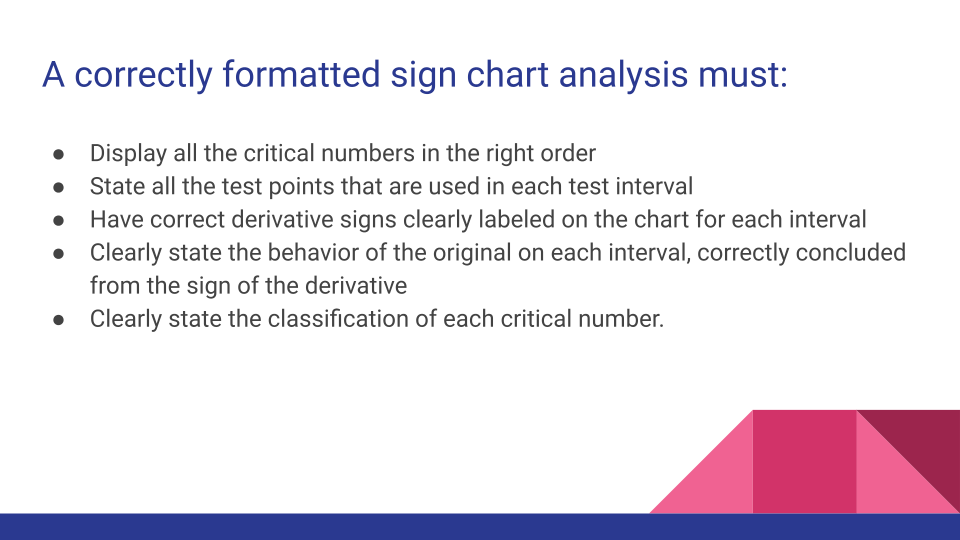
\includegraphics[width=0.5\textwidth]{signchart}
	\end{center}
	
	\item Fill in the blanks. Note that the intervals asked for here will depend on $a$, and so you should see an $a$ in the endpoints. 
	
	\begin{itemize}
		\item The function $f$ is increasing on the interval \blank.
		\item The function $f$ is decreasing on the interval \blank. 
	\end{itemize}
	
	\pageturn
	
	\item Use the information from the previous question to classify the critical values you found earlier as local minima, local maxima, or neither. 
	
	\begin{center}
		\begin{tabular}{c||c|c|c}
		Critical value & Sign of $f'$ just before  & Sign of $f'$ just after & Classification:  \\ \hline
		\hspace{0.5in} & \hspace{0.5in} & \hspace{0.5in} & \hspace{0.5in}  \\ \hline
		\hspace{0.5in} & \hspace{0.5in} & \hspace{0.5in} & \hspace{0.5in}  		
		\end{tabular}
	\end{center}
	
	
	\item Find $f''$ and use the result to complete a sign chart for $f''$ below. 
	\begin{center}
		\includegraphics[width=0.6\textwidth]{signchart-second}
	\end{center}
	
	
	\item Fill in the blanks. Do the intervals being asked for here depend on $a$ this time? 
	\begin{itemize}
		\item The function $f$ is concave up on the interval \blank.
		\item The function $f$ is concave down on the interval \blank. 
	\end{itemize}
	
	\item Find the inflection points of $f$. Do the locations of the inflection points depend on $a$? 
	 
	\vspace{0.5in}
	
\end{enumerate}


\section{A two-parameter family} 
Consider the two-parameter family of functions 
\[ h(x) = a(1- e^{-bx}) \] 
where $a,b > 0$ are constants. 

\begin{enumerate}
	\item (Mini-focus question) \ For what values of $x$ does $e^x = 0$? 
	\vspace{0.4in}
	
	\item Calculate $h'(x)$ and fully simplify your answer. (The result will include the parameters $a$ and $b$.) 
	
	\pageturn
	
	
	\item Find the critical values of $h$, if it has any. If it doesn't have any, say so and explain why. 
	\vspace{0.5in}
	
	\item On what interval or intervals is $h$ increasing? Decreasing? 
	\vspace{0.7in}
	
	
	\item Calculate $h''(x)$ and fully simplify your answer. (The result will include the parameters $a$ and $b$.) 
	\vspace{1in}
	
	\item On what interval or intervals is $h$ concave up? Concave down?
	\vspace{0.5in}
	
	
	\item What is the value of $\displaystyle{\lim_{x \to \infty} a(1-e^{-bx}) }$?  (Hint: First think about $\displaystyle{\lim_{x \to \infty} e^{-bx} }$ and remember $a$ and $b$ are constants, and do not depend on $x$.)
	\vspace{0.7in}
	
	\item Here is a Geogebra applet that lets you play with this family, using sliders to change the values of $a$ and $b$. You can pop up one of the computers in the room or use your own laptop, tablet, or smartphone to manipulate it: 
	\begin{center}
		\url{http://geogebratube.org/student/m40138}
	\end{center}
	Does this match what you found above through your mathematical work? 
	
	\item How does changing the value of $a$ affect the shape of the curve? How does changing the value of $b$ affect the shape of the curve? 
	
	
	
\end{enumerate}

\vfill 

\cuthere

\noindent
\textbf{A question I have after today's class work is:}

\vspace{1in}

\end{document}